\documentclass[12pt, a4paper]{article}

\usepackage{amsmath}
\usepackage{bm}
\usepackage{array}
\usepackage{amsmath}
\usepackage[portuguese]{babel}
\usepackage{chngpage}
\usepackage{float}
\usepackage[a4paper, margin=2cm]{geometry}
\usepackage{graphicx}
\usepackage{hyperref}
\usepackage{listings}
\usepackage{setspace}
\usepackage{xcolor}

\lstdefinestyle{codestyle}{
    commentstyle=\color{teal},
    keywordstyle=\color{blue},
    numberstyle=\ttfamily\color{gray},
    stringstyle=\color{red},
    basicstyle=\ttfamily\footnotesize,
    breakatwhitespace=false,
    breaklines=false,
    keepspaces=true,
    numbers=none,
    showspaces=false,
    showstringspaces=false,
    showtabs=false,
    tabsize=4
}
\lstset{style=codestyle}

\title{\Huge \textbf{Computação Gráfica \\ \Large Trabalho Prático -- Fase II}}
\date{30 de março 2025}
\author{Grupo 3}

\begin{document}

\begin{center}
    
\includegraphics[width=0.25\textwidth]{res/cover/EE-C.eps}
\end{center}

\chardef\_=`_
\onehalfspacing
\setlength{\parskip}{\baselineskip}
\setlength{\parindent}{0pt}
\def\arraystretch{1.5}

{\let\newpage\relax\maketitle}
\maketitle
\thispagestyle{empty}

\vspace*{\fill}

\begin{adjustwidth}{-2cm}{-2cm} % These values only need to be large enough to center the table
    \begin{center}
        \begin{tabular}{>{\centering}p{0.25\textwidth}
                        >{\centering}p{0.25\textwidth}
                        >{\centering}p{0.25\textwidth}
                        >{\centering\arraybackslash}p{0.25\textwidth}}
            
\includegraphics[width=3.5cm]{res/cover/A104437.png} &
            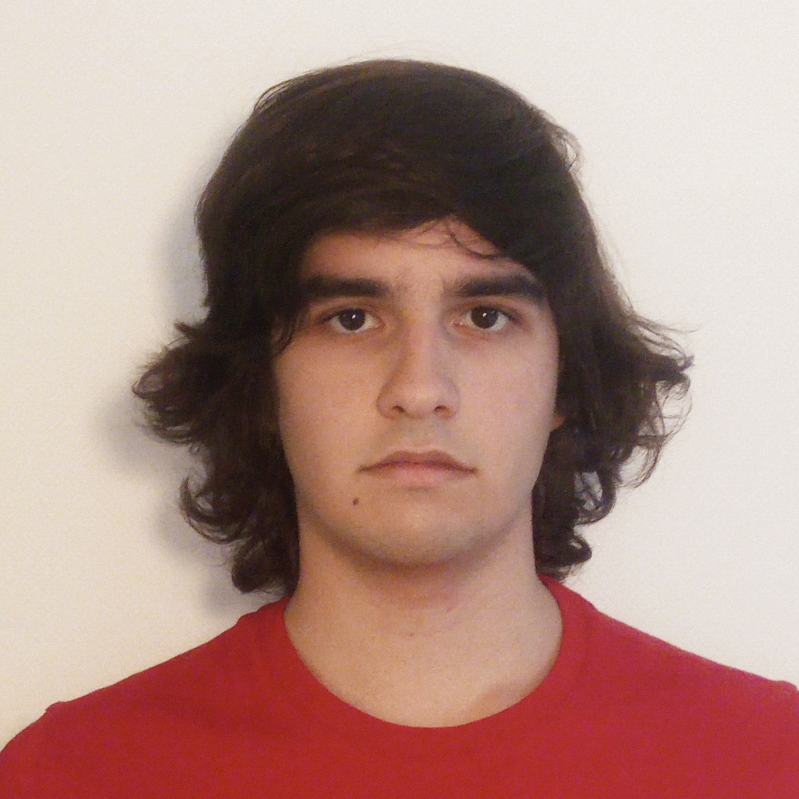
\includegraphics[width=3.5cm]{res/cover/A104348.png} &
            
\includegraphics[width=3.5cm]{res/cover/A90817.png} &
            
\includegraphics[width=3.5cm]{res/cover/A104179.png} \\

            Ana Oliveira & Humberto Gomes & Mariana Cristino & Sara Lopes \\
            A104437      & A104348        & A90817           & A104179
        \end{tabular}
    \end{center}
\end{adjustwidth}

\pagebreak

\begin{abstract}
    \textbf{\color{red} TODO - resumo}
\end{abstract}

\section{Transformações}

Um dos objetivos desta fase do trabalho prático é a possibilidade de aplicar transformações de
translação, rotação e escala às entidades na cena. Estas podem ser especificadas no ficheiro XML
como se apresenta no exemplo abaixo:

\lstset{language=xml}
\begin{lstlisting}

<group>
    <transform>
		<translate            x="1" y="2" z="3" />
        <rotate    angle="90" x="0" y="0" z="1" />
		<scale                x="1" y="2" z="1" />
    </transform>
    <models>
        <model file="modelo.3d" />
    </models>
</group>
\end{lstlisting}

Neste exemplo, a todos os modelos em \texttt{<models>} devem ser aplicadas, por esta ordem, uma
translação pelo vetor $(1, 2, 3)$, uma rotação de 90º pelo eixo $z$, e uma escala vertical por um
fator de duas vezes. Para calcular as matrizes associadas a cada uma destas transformações, as
funções \texttt{glm::translate}, \texttt{glm::rotate}, \texttt{glm::scale} são utilizadas.
\cite{glm-transform} Estas são semelhantes às funções \texttt{glTranslate}, \texttt{glRotate} e
\texttt{glScale} \cite{gl-transforms}, respetivamente, mas devolvem a matriz de transformação
calculada, em vez de modificarem as matrizes do estado interno do OpenGL. Outra diferença é que o
ângulo dado à função \texttt{glm::rotate} deve ser passado em radianos, sendo necessária uma
conversão do valor em graus presente na descrição XML da cena.

Para compor estas operações, as matrizes geradas pela \texttt{glm} são multiplicadas pela ordem em
que as transformações surgem no ficheiro XML. No exemplo anterior, onde $T$ é a matriz da
translação, $R$ a matriz de rotação, e $S$ a matriz de escala, as coordenadas no mundo dos pontos do
modelo devem ser multiplicadas pela matriz $W$ abaixo, originando as coordenadas no mundo do modelo
transformado:

$$
W = T R S
$$

Para desenhar as entidades no ecrã, é necessário também ter em conta a matriz da câmara, $C$, o
produto entre a matriz de projeção e a matriz de vista. Ademais, como os grupos na cena formam uma
hierarquia, é necessário considerar as transformações dos ascendentes de um grupo para o desenhar.
Assim, para desenhar a cena, usa-se uma \emph{stack} de matrizes, inicializada com a matriz da
câmara. Depois, para cada grupo aninhado, calcula-se o produto entre a matriz no topo do
\emph{stack} e a matriz de transformação do grupo, e esta matriz calculada é adicionada ao topo da
\emph{stack}. Quando se termina o desenho do grupo, é removida a matriz do topo da \emph{stack}. No
exemplo abaixo, mostra-se a \emph{stack} de matrizes durante o desenho de um grupo na hierarquia da
cena:

\begin{figure}[h]
    \begin{minipage}{0.5\textwidth}
        \centering
        \begin{tabular}{|>{\centering\arraybackslash}m{3cm}|}
            \hline \\
            \hline $C \cdot T_1 \cdot T_3 \cdot T_4$ \\
            \hline $C \cdot T_1 \cdot T_3$ \\
            \hline $C \cdot T_1$ \\
            \hline $C$ \\
            \hline
        \end{tabular}
    \end{minipage}
    \begin{minipage}{0.5\textwidth}
        \centering
        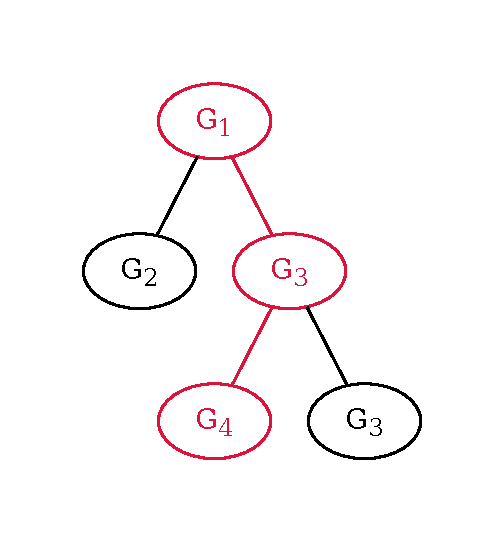
\includegraphics[width=0.6\textwidth]{res/phase2/SceneGraph.pdf}
    \end{minipage}
    \caption{\emph{Stack} de matrizes associada ao desenho de um grupo numa cena hierárquica.}
\end{figure}

\section{Sistema Solar Estático}

\subsection{Hierarquia do Sistema Solar}

O sistema solar foi representado através de uma estrutura hierárquica que segue a disposição
real
dos corpos celestes. No nível mais elevado encontra-se o Sol, que serve de ponto central e de
referência para a órbita dos restantes corpos celestes.

Cada planeta foi colocado num grupo independente, associado diretamente ao Sol. Quando aplicável,
os satélites naturais (luas) e os anéis são inseridos como grupos filhos do planeta
correspondente, preservando a hierarquia entre os corpos. A cintura de asteróides, por sua vez,
é representada como um grupo filho do Sol, uma vez que orbita em torno deste.

Desta forma, assegura-se que:
\begin{itemize}
    \item os planetas orbitam em torno do Sol;
    \item as luas orbitam em torno do planeta a que pertencem;
    \item os anéis acompanham o planeta respetivo;
    \item os asteróides se posicionam nas suas cinturas, em órbitas relativas ao Sol.
\end{itemize}

\subsection{Representação em XML}

A estrutura em XML segue a hierarquia descrita anteriormente. Cada grupo define transformações
aplicadas aos seus elementos, como \texttt{translate}, \texttt{rotate} e \texttt{scale}, que são
acumuladas ao longo da árvore de grupos. Esta organização permite simular corretamente os
movimentos
e proporções relativos entre os corpos celestes, como as órbitas dos planetas em torno do Sol
ou
das luas em torno dos seus planetas.

Abaixo apresenta-se um exemplo com o Sol, a Terra e a Lua:

\begin{lstlisting}
<group>
    <!-- Grupo do sol -->
    <group>
        <transform>
            <translate x="0" y="0" z="0"/>
            <scale x="30" y="30" z="30"/>
        </transform>
        <models>
            <model file="../models/sphere.3d"/>
        </models>
        <!-- Grupo do planeta Terra -->
        <group>
            <transform>
                <translate x="28" y="0" z="-3"/>
                <scale x="0.2" y="0.2" z="0.2"/>
            </transform>
            <models>
                <model file="../models/sphere.3d"/>
            </models>
            <!-- Grupo da lua -->
            <group>
                <transform>
                    <translate x="3" y="0" z="0"/>
                    <scale x="0.05" y="0.05" z="0.05"/>
                </transform>
                <models>
                    <model file="../models/sphere.3d"/>
                </models>
            </group>
        </group>
    </group>
</group>
\end{lstlisting}

Neste exemplo:
\begin{itemize}
    \item O primeiro \texttt{group} representa o Sol, posicionado na origem e aumentado com
    \texttt{scale}.
    \item Dentro do grupo do Sol encontra-se a Terra, posicionada com \texttt{translate} e
    redimensionada.
    \item Dentro do grupo da Terra está a Lua, com a sua própria transformação relativa.
\end{itemize}

As transformações são aplicadas sequencialmente e propagam-se ao longo da hierarquia. Assim, a
posição e a escala de cada corpo são relativas ao seu elemento pai, respeitando a estrutura do
sistema solar. Isto permite gerar movimentos orbitais e tamanhos proporcionais com base em
operações simples.

Além dos planetas e das luas, existem dois tipos de elementos adicionais com representação
específica no XML:

\begin{itemize}
    \item As \textbf{cinturas de asteróides} são compostas por figuras \texttt{sphere.3d},
    \texttt{box.3d} e \texttt{cylinder.3d}, escolhidas aleatoriamente. Estas instâncias são
    adicionadas como grupo filho do Sol e posicionadas com coordenadas aleatórias em torno de um
    raio definido. Cada asteróide recebe transformações próprias de \texttt{translate},
    \texttt{rotate} e \texttt{scale}, simulando a sua dispersão e dimensão variável.

    \item Os \textbf{anéis} reutilizam o modelo \texttt{torus.3d} da Fase I. Para
    simular a sua aparência achatada, é aplicada uma \texttt{scale} com fator reduzido no eixo
Y.
    Além disso, os anéis são orientados através de uma rotação (\texttt{rotate}) com
ângulo e
    eixo ajustados consoante o planeta. Cada anel é inserido como grupo filho do planeta
    correspondente.
\end{itemize}

O resultado destas pode ser visto na seguinte figura:

\begin{figure}[H]
    \centering
    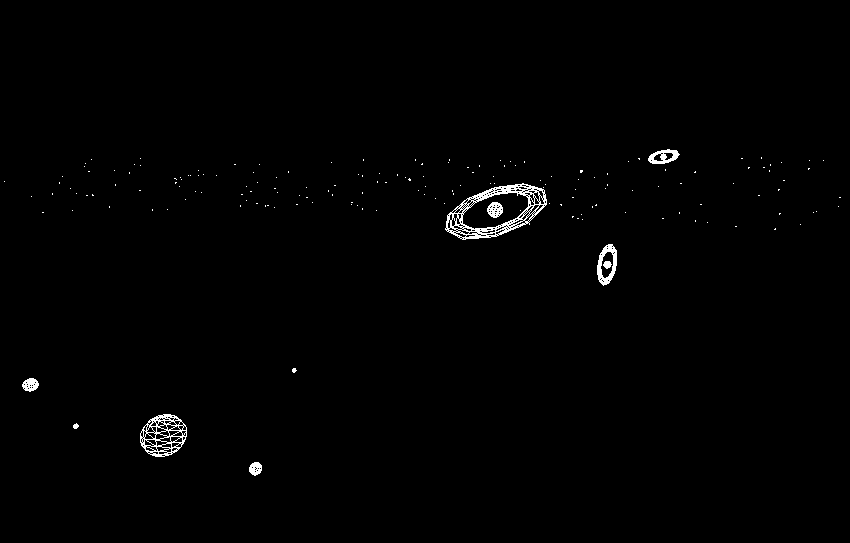
\includegraphics[width=0.9\linewidth]{res/phase2/results/SolarSystemOverview.png}
    \caption{Sistema solar com anéis e cinturas de asteróides visíveis.}
\end{figure}

Ainda existem muitas melhorias que podem ser feitas ao sistema solar, como movimento dos corpos
ou texturas.
Pretendemos implementa-las na próxima fase.

\subsection{Parametrização pelo Utilizador}

O sistema solar pode ser gerado de forma personalizada, atrvés dos seguintes parâmetros
definidos
pelo utilizador, via linha de comandos:

\begin{itemize}
    \item \texttt{sceneScale} — Escala global aplicada a toda a cena.
    \item \texttt{sunSizeFactor} — Escala atribuída ao Sol.
    \item \texttt{planetSizeFactor} — Escala definida para os planetas.
    \item \texttt{moonSizeFactor} — Escala definida para os satélites naturais.
    \item \texttt{distanceFactor} — Proporção da distância entre os diferentes corpos
celestes.
    \item \texttt{asteroidBeltDensity} — Densidade definida para as cinturas de asteróides.
    \item \texttt{ringSizeFactor} — Proporção dos anéis em relação ao planeta.
\end{itemize}

O objetivo destes parâmetros é gerar modelos do sistema solar com diferentes escalas e
proporções, para facilitar a experiência do utilizador.

\section{Extras}

\subsection{Câmara Orbital}

A câmara orbital é uma câmara virtual que permite observar uma scene a partir de um ponto que
orbita à volta de um objeto ou de um ponto de vista (\texttt{lookAt}). Na implementação atual, este
ponto de interesse está fixado na origem do espaço tridimensional. Esta abordagem é útil para
observar um objeto de diversos ângulos possíveis com o foco num ponto em específico.

\subsubsection{Movimentação e Controlo}

A câmara orbital é definida por 3 parâmetros:
\begin{itemize}
    \item Raio (\texttt{radius}): determina a distância do ponto de interesse à câmara;
    \item Ângulo azimutal ($\phi$): define a rotação da câmara em torno do eixo vertical,
    o que permite uma visualização de 360 graus ao redor do objeto;
    \item Ângulo polar ($\theta$): controla o ângulo de elevação da câmara.
\end{itemize}

A atualização da a posição da câmara é dada pela soma do ponto de interesse (\texttt{lookAt}) com
as coordenadas cartesianas obtidas a partir das coordenadas esféricas. As fórmulas utilizadas para
a conversão são as seguintes:

$$x = radius \times \sin(\theta) \times \cos(\phi)$$
$$y = radius \times \cos(\theta)$$
$$z = radius \times \sin(\theta) \times \sin(\phi)$$

De forma a garantir um comportamento estável e consistente, os valores são restringidos a
intervalos pré-definidos. O raio encontra-se limitado entre $0.5$ e $100$, para evitar que a câmara
se aproxime demasiado ou se afaste demasiado do ponto de interesse. O ângulo azimutal varia entre
$0$ e $2\pi$, para que a rotação aconteça de forma contínua. Por fim, o ângulo polar encontra-se
entre $0.01$ e $\pi - 0.01$ para evitar que a câmara alcance os polos e cause instabilidade no
movimento, no sentido em que se $\theta$ atingir o valor $\pi$, o vetor \texttt{up} da câmara
ficaria invertido, de modo que a câmara viraria completamente ao contrário. Assim, os comandos
também ficariam invertidos, isso tornaria a navegação confusa e pouco intuitiva.

\subsubsection{Controlo pelo Utilizador}

Para controlar a câmara orbital, o utilizador utiliza o teclado, sendo que as teclas associadas a
cada ação são:
\begin{itemize}
    \item \texttt{W}: inclina a câmara para cima;
    \item \texttt{S}: inclina a câmara para baixo;
    \item \texttt{A}: roda a câmara para a esquerda;
    \item \texttt{D}: roda a câmara para a direita;
    \item \texttt{F}: aproxima a câmara do ponto de interesse;
    \item \texttt{B}: afasta a câmara do ponto de interesse.
\end{itemize}

\subsection{Garrafa de Klein}

A garrafa de Klein é uma superfície não orientável, ou seja, não possui um lado interno e externo
distinguíveis. Esta não possui fronteira e trata-se de uma variedade bidimensional onde não se pode
definir um vetor normal em todos os pontos.

\subsubsection{Geração dos vértices}

A parametrização de um vértice sobre a garrafa de klein de raio $r$ pode ser definida pelas
seguintes equações \cite{bottleKlein}:

$$
x = r \left( \frac{-2}{15} \right) \cos(\theta) \left(3 \cos(\phi) - 30 \sin(\theta) +
90 \cos^4(\theta) \sin(\theta) - 60 \cos^6(\theta) \sin(\theta) +
5 \cos(\theta) \cos(\phi) \sin(\theta) \right)
$$

$$
y = r \left( \frac{-1}{15} \right) \sin(\theta) \left( 3 \cos(\phi) - 3 \cos^2(\theta) \cos(\phi)
- 48 \cos^4(\theta) \cos(\phi) + 48 \cos^6(\theta) \cos(\phi) - 60 \sin(\theta) \right.
$$
$$
\quad \left. + 5 \cos(\theta) \cos(\phi) \sin(\theta) - 5 \cos^3(\theta) \cos(\phi) \sin(\theta)
- 80 \cos^5(\theta) \cos(\phi) \sin(\theta) + 80 \cos^7(\theta) \cos(\phi) \sin(\theta) \right)
$$

$$
z = r \left( \frac{2}{15} \right) (3 + 5 \cos(\theta) \sin(\theta)) \sin(\phi)
$$

Para a geração da garrafa de Klein, a superfície foi discretizada com a utilização de coordenadas
paramétricas, com o auxílio de duas variáveis ($\theta$ e $\phi$).

A variável $\theta$ varia entre $0$ e $\pi$ e $\phi$ varia entre $0$ e $2\pi$. Além disso, o
intervalo de valores de $\theta$ e $\phi$ varia de acordo com o número de slices e stacks.

\subsubsection{Construção das faces}

Após a geração dos vértices, constroem-se as faces da garrafa de Klein. Cada quadrilátero entre duas
\emph{stacks} sucessivas é dividido em duas faces triangulares.

\begin{figure}[H]
    \centering
    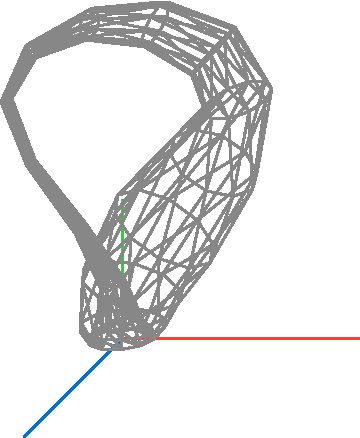
\includegraphics[width=0.3\textwidth]{res/phase2/figures/kleinBottle.pdf}
    \caption{Garrafa de Klein}
\end{figure}

\subsection{Roda Dentada}

A roda dentada é uma derivaçaão do cilindro, na medida em que possui uma estrutura básica
cilíndrica, no entanto tem o complemento dos dentes no exterior e uma coroa no interior. A
construção desta primitiva tem por base coordenadas cilíndricas, onde a posição de cada ponto é
dada pelo raio interno ($r_i$), raio externo ($r_e$), ângulo azimutal ($\phi$) e altura ($h$).

A parametrização de um ponto sobre uma roda dentada de raio \( r \) pode ser definida
pelas seguintes equações:

$$x = r \cos(\phi)$$
$$y \in \left [ 0, h \right ]$$
$$z =  r \sin(\phi)$$


onde $r$ possui dois valores distintos. Para a parte interna da roda é utilizado o $r_i$ e para a
parte externa o $r_e$. Os dentes são gerados na circunferência exterior, com o aumento do raio em
determinadas posições.

\subsubsection{Geração dos Vértices}

Para discretizar a superfície da roda dentada, divide-se o intervalo de $\phi$ em \emph{slices}, e
o intervalo de $y$ em \emph{stacks}. Assim, as incrementações angulares são calculadas da seguinte
forma:

$$
\Delta \phi = \frac{2\pi}{N_\text{slices}}
\hspace{1cm}
\Delta y = \frac{h}{N_\text{stacks}}
$$

A construção dos vértices segue os seguintes passos:

1. Superfície lateral externa: Para cada \emph{stack}, os valores de $\phi$ são iterados,
determinando a posição dos pontos ao longo da circunferência externa. Nos intervalos correspondentes
aos dentes, o raio é aumentado em $r_e + h_t$, onde $h_t$ é a altura do dente.

2. Superfície lateral interna: De forma similar à superfície lateral externa, é gerada a superfície
interna do cilindro, mas o raio mantém-se constante em $r_i$.

\subsubsection{Construção das Faces}

Após a geração dos vértices, é necessário definir as faces triangulares que compõem a roda dentada.
A triangulação é realizada da seguinte forma:

1. Superfície lateral externa: Os pontos adjacentes de duas \emph{stacks} consecutivas são
ligados, isto forma quadriláteros que são divididos individualmente em dois triângulos.

2. Superfície lateral interna: É aplicada a mesma estratégia ao cilindro interno, com a ligação
dos pontos entre diferentes \emph{stacks}.

3. Bases superior e inferior: Os pontos da última \emph{stack} são ligados ao vértice central
correspondente, de modo a formar triângulos radiais.

\begin{figure}[H]
    \centering
    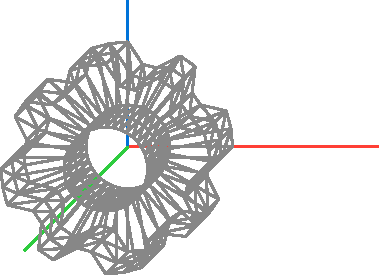
\includegraphics[width=0.3\textwidth]{res/phase2/figures/gear.pdf}
    \caption{Representação da estrutura da roda dentada.}
\end{figure}

\subsection{UI (Interface Gráfica)}

A interface do projeto foi desenvolvida com o auxílio da biblioteca \texttt{Dear ImGui}. Esta
biblioteca simplifica a gestão e atualização dos componentes, pois os elementos gráficos são
recriados a cada \textit{frame}.

A classe responsável pela configuração e renderização da interface é a \texttt{UI}.
Assim, no processo de inicialização realizado no construtor da classe, a criação do contexto
\texttt{ImGui} é realizada (garante que a biblioteca encontra-se bem configurada), bem como a
configuração do estilo da interface (aqui, o estilo \textit{Dark} foi escolhido para se obter uma
melhor visualização dos elementos gráficos) e é efetuada a inicialização das implementações para a
\texttt{OpenGL} e \texttt{GLFW} (assegura que há compatibilidade entre o motor de renderização
utilizado com o sistema de janelas).

A interface é composta por um menu, sendo este renderizado na função \texttt{UI::render} com os
seguintes elementos:

\begin{itemize}
    \item Acompanhamento do Desempenho:
    \begin{itemize}
        \item FPS (\textit{Frames Per Second}): apresenta o número de \textit{frames}
        renderizados por segundo.
        \item Apresenta o número de entidades renderizadas em relação ao número total de entidades
        existentes. Esta métrica é útil para testar a eficiência do \textit{frustum culling},
        pois permite avaliar se apenas as entidades dentro da visão da câmara estão a ser
        renderizadas.
    \end{itemize}
    \item Configurações:
    \begin{itemize}
        \item Preenchimento de polígonos: permite alternar entre o preenchimento
        (\textit{fill polygons}) e o modo \textit{wireframe}.
        \item \textit{Back face culling}: ativa ou desativa o \textit{back-face culling}.
        \item Exibir eixos: ativa ou desativa a visualização dos eixos.
        \item \textit{Bounding spheres}: ativa ou desativa a visualização das esferas encapsuladoras
        das entidades.
    \end{itemize}
    \item Câmara: permite modificar as coordenadas da posição da câmara.
\end{itemize}

Após a definição dos elementos gráficos, a interface é renderizada através das funções
\texttt{ImGui::Render} e \texttt{ImGui\_ImplOpenGL3\_RenderDrawData}.

\begin{figure}[H]
    \centering
    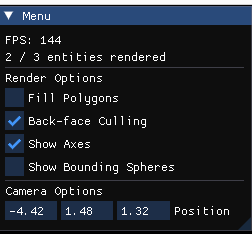
\includegraphics[width=0.35\textwidth]{res/phase2/UI.png}
    \caption{Interface Gráfica.}
\end{figure}

\section{\emph{Frustum culling}}

Cada \emph{draw call} tem um custo elevado para o desempenho da aplicação. Logo, procurando reduzir
o número de \emph{draw calls}, foi implementado \emph{frustum culling}, para apenas ser requisitada
à GPU a renderização das entitidades totalmente ou parcialmente no \emph{view frustum} da câmara.

Seria muito computacionalmente intensivo verificar se a geometria de um modelo se encontra dentro ou
fora do \emph{view frustum}, pelo que se encapsulam todos os modelos em esferas que, devido à sua
geometria simples, permitem uma verificação rápida da sua visibilidade no \emph{view frustum}. No
entanto, visto que estas esferas podem ser um pouco maiores do que os modelos em si, é possível que
algumas entidades fora do ecrã sejam desenhadas, visto que parte das suas esferas ainda podem
intersetar os planos do \emph{view frustum}. Para mitigar este problema, formas geométricas
encapsuladoras mais complexas poderiam ser utilizadas, visto que estas se poderiam adaptar melhor à
geometria dos modelos. No entanto, o uso destas formas complexas conduziria a testes de visibilidade
mais caros, possivelmente anulando os benefícios de desenhar um menor número de entidades.

Quando um modelo é carregado, é necessário calcular a esfera que o encapsula. Em primeiro lugar, o
seu centro é calculado como o centro de massa de todos os pontos, como mostra a expressão abaixo,
onde $M$ é o modelo, uma sequência de pontos tridimensionais:

$$
C = \frac{1}{|M|} \sum_{p \in M} p
$$

Depois, o raio da esfera pode ser determinado como a distância entre o centro da esfera e o ponto
mais longínquo do mesmo, como mostra a expressão abaixo, onde $d$ é a função de distância cartesiana
entre dois pontos:

$$
r = \max \left \lbrace d(C, p) \mid p \in M \right \rbrace
$$

É também necessário saber como uma esfera encapsuladora é afetada quando o objeto que encapsula
sofre uma transformação no mundo. Considere-se uma matriz de transformação aplicada ao objeto (em
coordenadas do mundo), originada através da aplicação de translações, rotações, e escalas. A matriz
será 4x4 e terá o seguinte aspeto:

$$
\bgroup
    T =
    \begin{bmatrix}
        \vec \imath & \vec \jmath & \vec k & \vec t \\
        0 & 0 & 0 & 1
    \end{bmatrix}
\egroup
$$

Para calcular o centro da esfera após a transformação da entidade, basta multiplicar a matriz de
transformação pela posição do centro da esfera:

$$
C' = T C
$$

Depois, para calcular o novo raio da esfera, não é necessário ter em conta as transformações de
rotação, visto que as esferas são simétricas em todos os eixos possíveis. No entanto, é necessário
ter em conta a escala aplicada ao modelo. Por exemplo, na matriz $T$, a escala da entidade pelo
eixo $x$ é $\lVert \vec \imath \rVert$, e o mesmo se tem para o eixo $y$ e
$\lVert \vec \jmath \rVert$, e para $z$ e $\lVert \vec k \rVert$. Logo, o raio da esfera
transformada é:

$$
r' =
    \max
        \left ( \lVert \vec \imath \rVert, \lVert \vec \jmath \rVert, \lVert \vec k \rVert \right )
    \cdot
        r
$$

É possível tirar proveito da estrutura hierárquica da cena para otimizar o processo de
\emph{frustum culling}. Por exemplo, caso um grupo contenha várias entidades ou subgrupos, pode
construir-se uma esfera que encapsula a totalidade do grupo. Caso essa esfera não esteja no
\emph{view frustum}, pode-se evitar fazer os testes de visibilidade para as esferas dos objetos
individuais que compõem o grupo. Caso contrário, é na mesma necessário realizar esses testes.

O processo para determinar as características de uma esfera que encapsula todos os objetos de um
grupo é semelhante ao da construção de esferas com base no conjunto de pontos de um modelo. Em
primeiro lugar, para determinar o centro da esfera, calcula-se o centro de massa do conjunto de
pontos formado pelos centros de todas as esferas, $C$. De seguida, para cada subesfera, calcula-se
a sua distância máxima a $C$, o raio da subesfera adicionado à distância entre $C$ e o centro da
subesfera. Depois, a maior destas distâncias é escolhida para ser o raio da nova esfera, como mostra
a expressão abaixo, onde $S$ representa o conjunto de subesferas:

$$
r' = \max \left \lbrace d(C', C) + r \mid (C, r) \in S \right \rbrace
$$

Depois de saber como determinar as esferas encapsuladoras das entidades, é necessário determinar
o \emph{view fustum} da câmara, para se poder verificar a posição das esferas em relação aos planos
do \emph{view fustum}. Para determinar o \emph{view frustum}, é necessário obter alguns vetores
importantes da câmara \cite{lighthouse3d-frustum-planes}:

\textbf{\color{red} TODO - com a fusão das partes do relatório, referenciar vetores da câmara livre}

Além destes vetores, é também necessário conhecer as dimensões dos planos \emph{near} e \emph{far}.
Apesar de, matematicamente, planos não terem uma altura e uma largura, utiliza-se esta linguagem
para se referir às dimensões dos retângulos nestes planos que constituem o \emph{view frustum}. Na
expressão abaixo, mostra-se como se pode calcular a altura ($H_\text{near}$) e a largura
($W_\text{near}$) do plano \emph{near}. O processo para o plano \emph{far} é semelhante. Com o FOV
da câmara ($\theta$), a distância ao plano \emph{near} ($d_\text{near}$) e o \emph{aspect ratio}
(A), podem calcular-se as dimensões deste plano \cite{lighthouse3d-frustum-distances}:

$$
H_\text{near} = 2 d_\text{near} \tan \left ( \frac{\theta}{2} \right )
\hspace{1cm}
W_\text{near} = H_\text{near} A
$$

Com estes valores, é possível determinar as coordenadas dos pontos dos retângulos do
\emph{view frustum}. Os quatro pontos do plano \emph{near} (a amarelo na figura abaixo) podem ser
calculados do seguinte modo, e o método utilizado para o plano \emph{far} é semelhante
\cite{lighthouse3d-frustum-planes}:

$$
F = P +
    d_\text{near} \; \widehat{d} \; \pm
    \frac{H_\text{near}}{2} \; \widehat{up} \; \pm
    \frac{W_\text{near}}{2} \; \widehat{r} \;
$$

\begin{figure}[H]
    \centering
    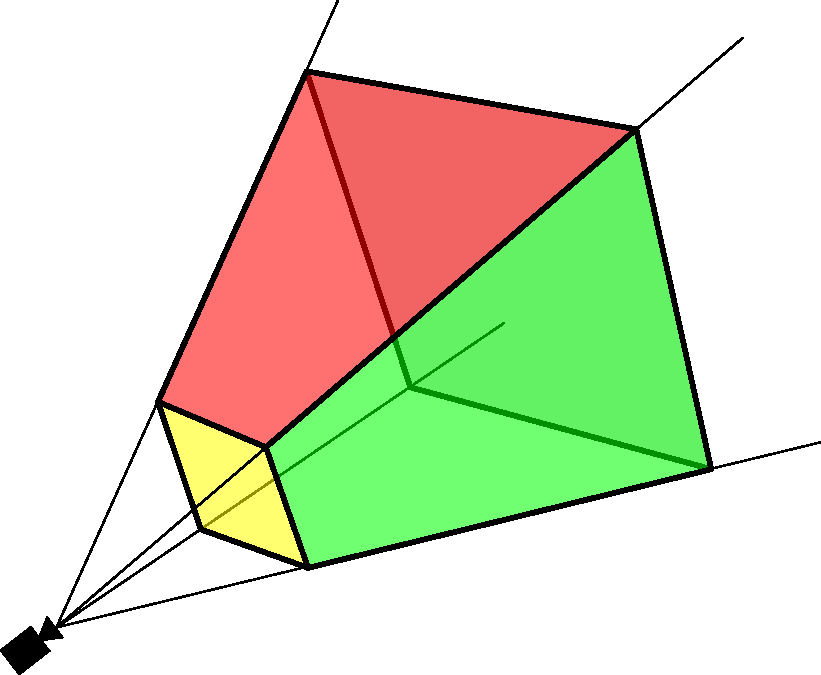
\includegraphics[width=0.4\textwidth]{res/phase2/ViewFrustum.pdf}
    \caption{\emph{View Frustum}.}
\end{figure}

Com os oito pontos do \emph{view frustum}, é possível determinar as equações cartesianas de cada
um dos seus planos, considerando três pontos da sua superfície. Em primeiro lugar, determina-se o
vetor normal ao plano. Com os três pontos, $P_1$, $P_2$ e $P_3$, determinam-se dois vetores, a
partir dos quais se calcula um produto externo, determinando-se assim um vetor perpendicular ao
plano \cite{lighthouse3d-plane}:

$$
n = \overrightarrow{P_1 P_2} \times \overrightarrow{P_1 P_3}
$$

Depois, com este vetor normalizado, é possível determinar a constante na equação cartesiana do plano
com base nas coordenadas de um dos três pontos dados \cite{lighthouse3d-plane}:

\begin{align*}
                       & \alpha x + \beta y + \gamma z + \delta = 0 \\
    \Leftrightarrow \; & \widehat{n} \cdot P + \delta = 0 \\
    \Leftrightarrow \; & \delta = -\widehat{n} \cdot P
\end{align*}

Durante a renderização de cada \emph{frame}, verificam-se que esferas estão totalmente ou
parcialmente dentro do \emph{view frustum}. Para uma esfera estar no \emph{view frustum} $F$, é
necessário que a distância assinada entre o centro da esfera e cada um dos planos do
\emph{view frustum} não seja inferior ao simétrico do seu raio, ou seja \cite{lighthouse3d-sphere}:

$$
\forall_{p \in F} \left ( \widehat{n} \cdot C + \delta \ge - r \right )
$$

Uma vez que é necessário calcular distâncias assinadas, é imperativo que os vetores normais de todos
os planos do \emph{view frustum} apontem para o seu interior, para que o conteúdo no seu interior (e
não no seu exterior) seja desenhado. \cite{lighthouse3d-frustum-planes} Por este motivo, a ordem em
que os pontos $P_1$, $P_2$ e $P_3$ são especificados é relevante.

\section{Resultados obtidos}

Nesta fase, implementámos câmaras orbital e livre, transformações hierárquicas, frustum culling e
novas primitivas geométricas. Os resultados incluem novos modelos de primitivas gerados pelo
\texttt{generator}, testes de renderização, uma representação funcional do sistema solar e a
implementação de \textit{frustum culling}.

\subsection{Figuras geométricas geradas}

Os seguintes modelos foram criados utilizando o \texttt{generator} implementado:

\begin{figure}[H]
    \centering
    \begin{minipage}{0.48\textwidth}
        \centering
        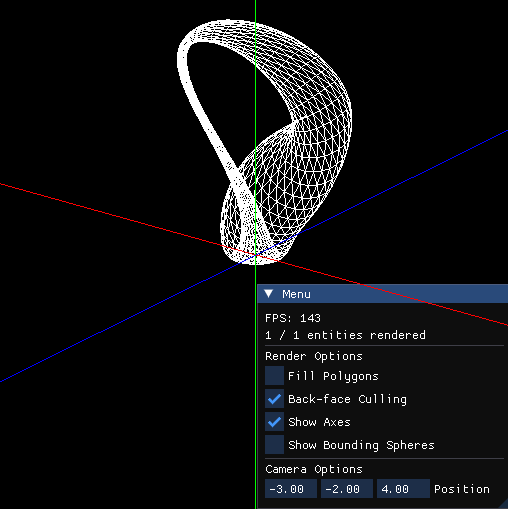
\includegraphics[width=0.5\textwidth]{res/phase2/results/KleinBottle.png}
        \caption{Garrafa de Klein (\texttt{kleinBottle})}
    \end{minipage}\hfill
    \begin{minipage}{0.48\textwidth}
        \centering
        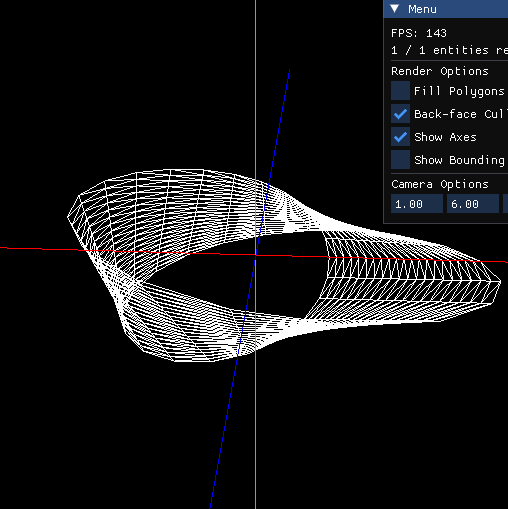
\includegraphics[width=0.5\textwidth]{res/phase2/results/MobiusStrip.png}
        \caption{Fita de Möbius (\texttt{möbius strip})}
    \end{minipage}
\end{figure}

\begin{figure}[H]
    \centering
    \begin{minipage}{0.48\textwidth}
        \centering
        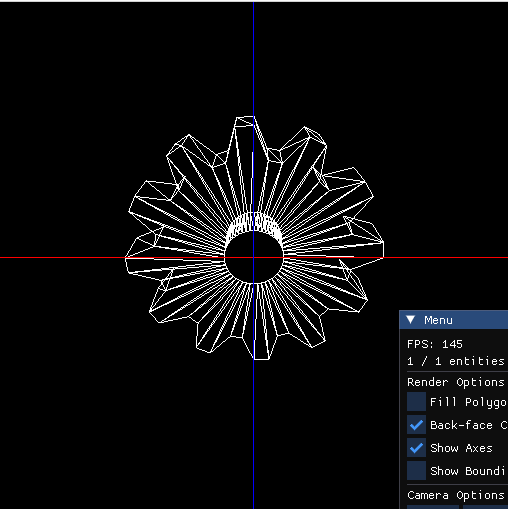
\includegraphics[width=0.5\textwidth]{res/phase2/results/Gear.png}
        \caption{Roda dentada (\texttt{gear})}
    \end{minipage}\hfill
\end{figure}

\subsection{Cenas fornecidas pela docência da UC}

A docência da UC forneceu, juntamente com o enunciado do trabalho, algumas cenas a serem testadas no
trabalho. A \texttt{engine} renderizou-as como esperado:

\begin{figure}[H]
    \begin{adjustwidth}{-2cm}{-2cm}
        \centering
        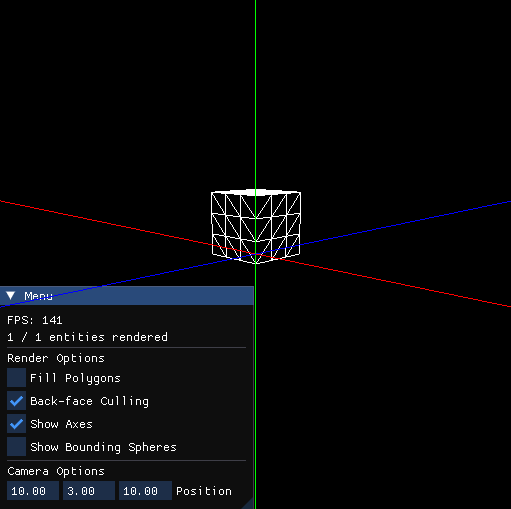
\includegraphics[width=0.26\textwidth]{res/phase2/results/Test1.png}
        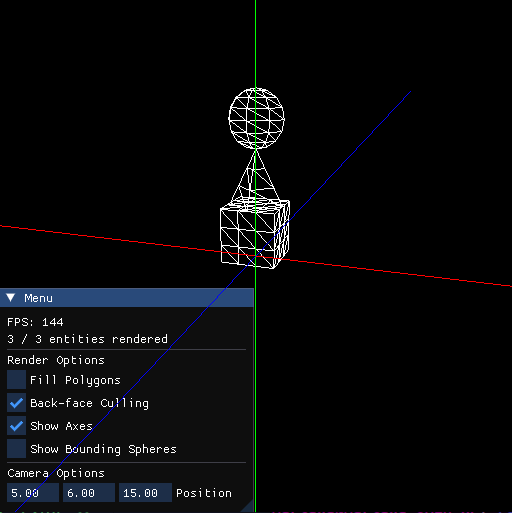
\includegraphics[width=0.26\textwidth]{res/phase2/results/Test2.png}
        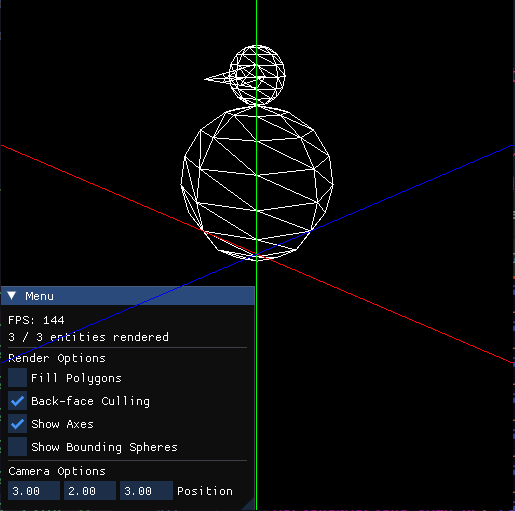
\includegraphics[width=0.26\textwidth]{res/phase2/results/Test3.png}
        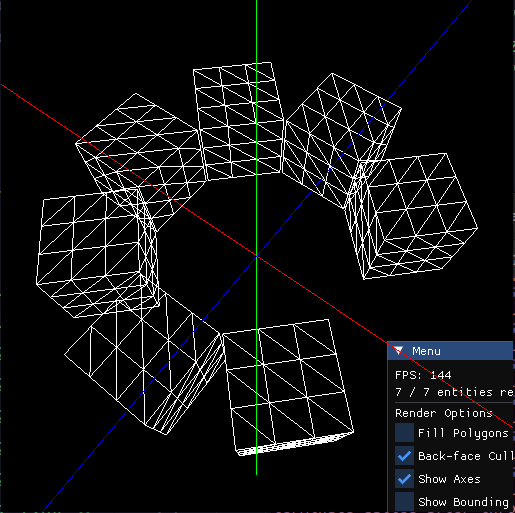
\includegraphics[width=0.26\textwidth]{res/phase2/results/Test4.png}
        \caption{Renderização das cenas de teste fornecidas pela docência da UC.}
    \end{adjustwidth}
\end{figure}

\subsection{Sistema Solar}

A hierarquia implementada produziu com sucesso as órbitas e relações de escala do sistema solar.

\begin{figure}[H]
    \centering
    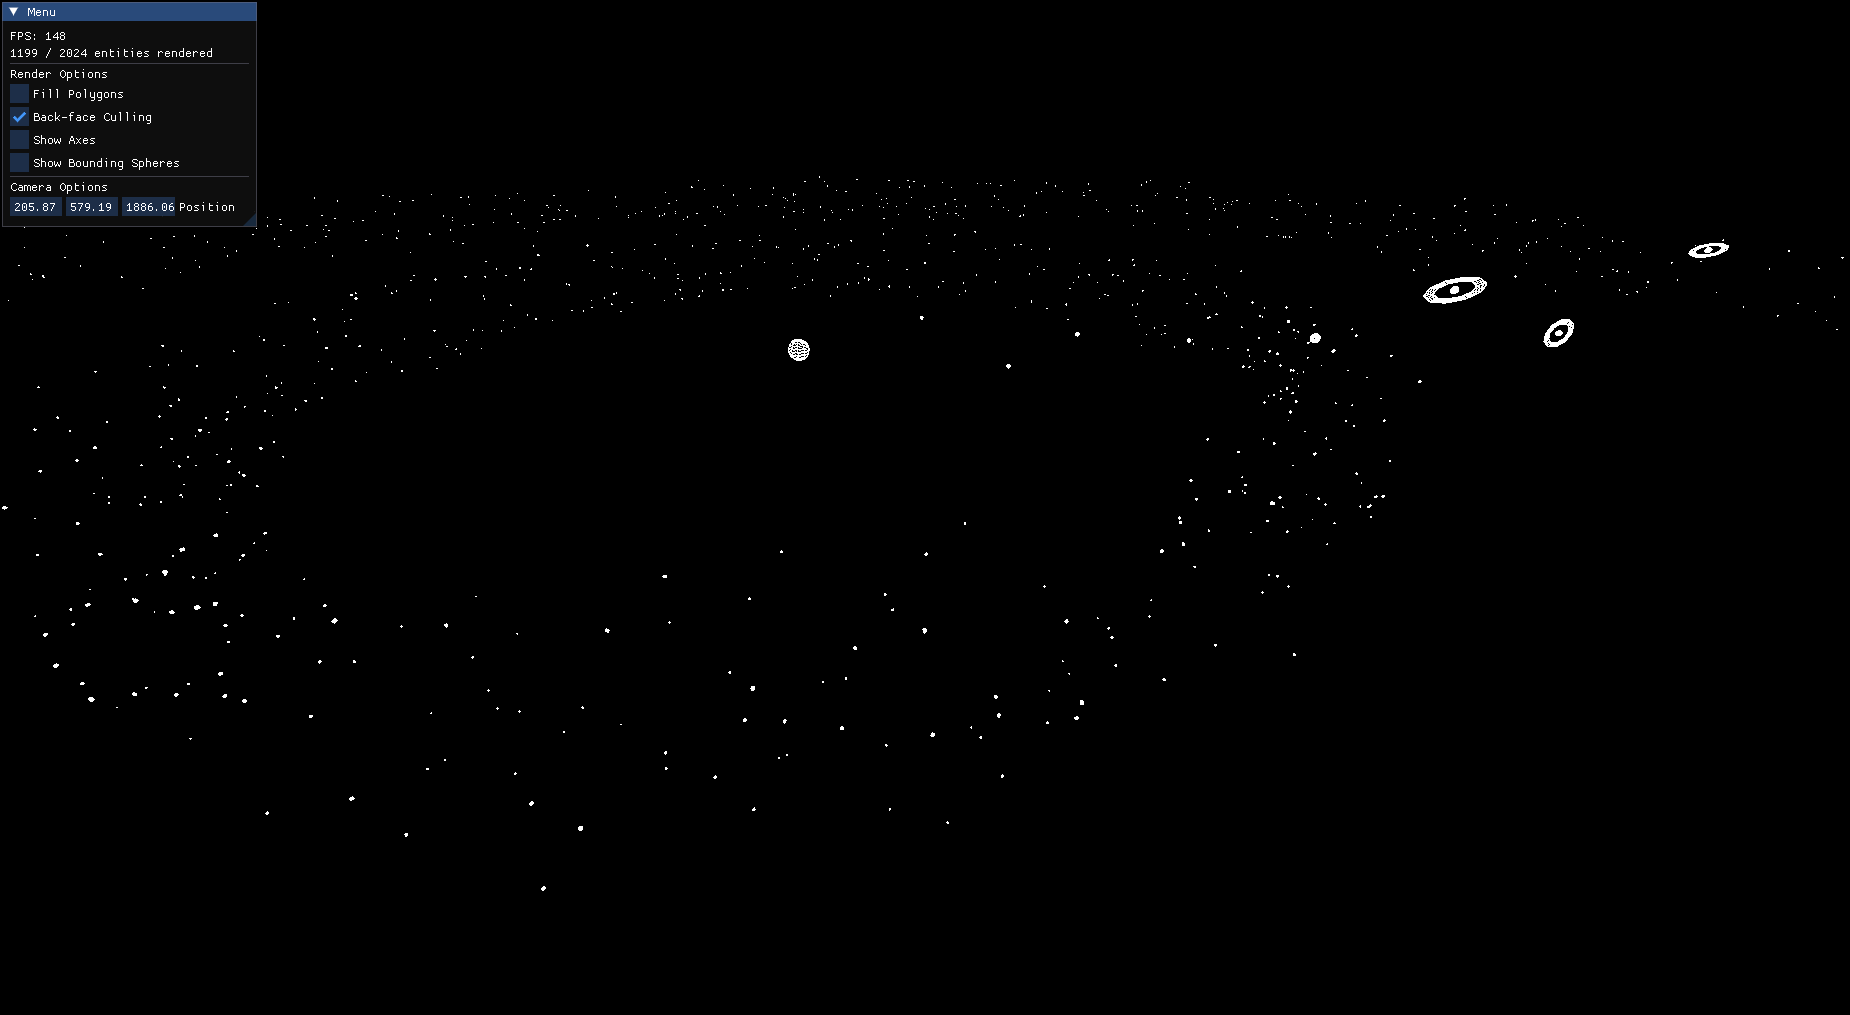
\includegraphics[width=0.5\textwidth]{res/phase2/results/SolarSystem.png}
    \caption{Renderização do sistema solar.}
\end{figure}

\subsection{Frustum Culling}

O \textit{frustum culling} utiliza as esferas vermelhas para verificar se um objeto
se encontra dentro do campo de visão da câmara. Se a esfera estiver dentro da área visível, o
modelo correspondente é renderizado. Os objetos que se encontrem fora do \textit{frustum} têm as
suas esferas ignoradas, o que evita um processamento desnecessário.

\begin{figure}[H]
    \begin{adjustwidth}{-2cm}{-2cm}
        \centering
        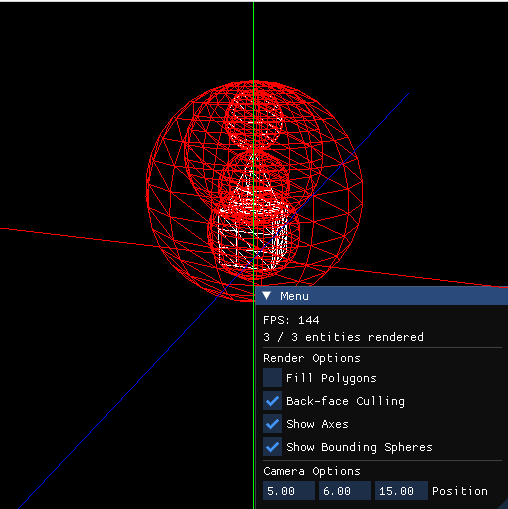
\includegraphics[width=0.4\textwidth]{res/phase2/results/FrustumCulling.png}
        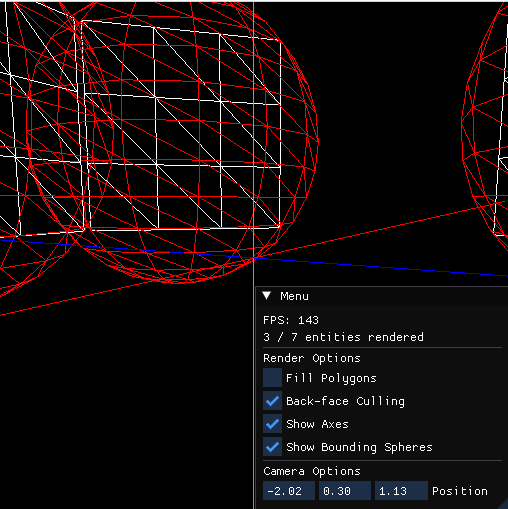
\includegraphics[width=0.4\textwidth]{res/phase2/results/FrustumCullingpt2.png}
        \caption{Frustum Culling}
    \end{adjustwidth}
\end{figure}

\section{Conclusão e Trabalho Futuro}

\textbf{\color{red} TODO - conclusão}

\begingroup
\section{Bibliografia}
\renewcommand{\section}[2]{}

\begin{thebibliography}{9}
    \bibitem{bottleKlein}
        "Klein bottle"{} Mathematics: Mar. 28, 2025. [Online.] Available:
     \url{https://math.stackexchange.com/questions/2982429/whats-the-surface-area-of-a-klein-bottle}
    \bibitem{Dear ImGui}
        "Dear ImGui."{} GitHub. Accessed: Mar. 2, 2025. [Online.] Available:
        \url{https://github.com/ocornut/imgui}
    \bibitem{glm-transform}
        ``GLM\textunderscore EXT\textunderscore matrix\textunderscore transform''. GLM 0.9.9 API
        documentation. Accessed: Mar. 27, 2025. [Online.] Available:
        \url{https://glm.g-truc.net/0.9.9/api/a00247.html}
    \bibitem{gl-transforms}
        ``OpenGL (R) 2.1, GLX, and GLU Reference Pages ''. Khronos Registry.
        Accessed: Mar. 27, 2025. [Online.] Available:
        \url{https://registry.khronos.org/OpenGL-Refpages/gl2.1}
    \bibitem{lighthouse3d-frustum-planes}
        ``Geometric Approach -- Extracting the Planes.''. Lighthouse3d.com. Accessed:
        Mar. 29, 2025. [Online.] Available:
        \url{https://www.lighthouse3d.com/tutorials/view-frustum-culling/geometric-approach-extracting-the-planes/}
    \bibitem{lighthouse3d-frustum-distances}
        ``View Frustum’s Shape.''. Lighthouse3d.com. Accessed:
        Mar. 29, 2025. [Online.] Available:
        \url{https://www.lighthouse3d.com/tutorials/view-frustum-culling/view-frustums-shape/}
    \bibitem{lighthouse3d-plane}
        ``Plane.''. Lighthouse3d.com. Accessed:
        Mar. 29, 2025. [Online.] Available:
        \url{https://www.lighthouse3d.com/tutorials/maths/plane/}
    \bibitem{lighthouse3d-sphere}
        ``Geometric Approach -- Testing Points and Spheres.''. Lighthouse3d.com. Accessed:
        Mar. 29, 2025. [Online.] Available:
        \url{https://www.lighthouse3d.com/tutorials/view-frustum-culling/geometric-approach-testing-points-and-spheres/}
\end{thebibliography}
\endgroup

\end{document}
